\documentclass{beamer}
%\usepackage[latin1]{inputenc}
%\usepackage{lmodern}
\usepackage{times}
\usepackage[T1]{fontenc}
\usepackage{graphicx}
\usepackage{bm}
\usepackage{tikz}
\usepackage{verbatim}
\usepackage{amsmath}
\usepackage[small,labelformat=empty]{caption}
\usepackage{url}
\usetikzlibrary{automata,positioning}

\usetheme{Frankfurt}
%\usetheme{Warsaw}
\title[Title of presentation]{Title of presentation\\
{\small possibly subtitle}
}
\author[author name]
{further information <\url{can-include.urls}>}
\institute[Fnord GmbH]{}
\date{23.5.1984 - 42.5.1984}

\begin{document}

\begin{frame}{Overview}
	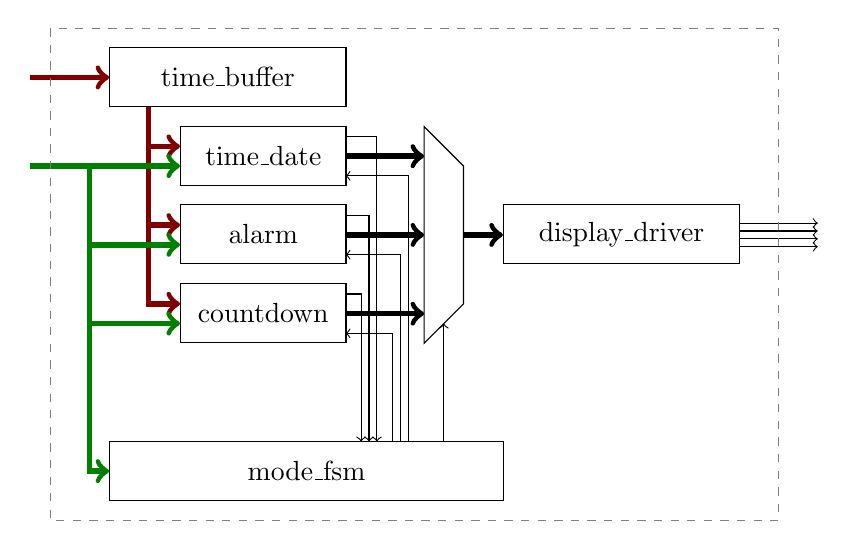
\begin{tikzpicture}
		% individual modules
		\node[rectangle,draw=black,minimum height=.75cm,minimum width=3cm,above right] at (0,-1) {time\_buffer};
		\node[rectangle,draw=black,minimum height=.75cm,minimum width=2.1cm,above right] at (.9,-2) {time\_date};
		\node[rectangle,draw=black,minimum height=.75cm,minimum width=2.1cm,above right] at (.9,-3) {alarm};
		\node[rectangle,draw=black,minimum height=.75cm,minimum width=2.1cm,above right] at (.9,-4) {countdown};
		\node[rectangle,draw=black,minimum height=.75cm,minimum width=3cm,above right] at (5,-3) {display\_driver};
		\node[rectangle,draw=black,minimum height=.75cm,minimum width=5cm,above right] at (0,-6) {mode\_fsm};

		% time signals
		\draw[red!50!black,line width=2pt,->] (-1,-.625) -- (0,-.625);
		\draw[red!50!black,line width=2pt,->] (.5,-1) -- (.5,-1.5) -> (.9,-1.5);
		\draw[red!50!black,line width=2pt,->] (.5,-1) -- (.5,-2.5) -> (.9,-2.5);
		\draw[red!50!black,line width=2pt,->] (.5,-1) -- (.5,-3.5) -> (.9,-3.5);

		% key status signals
		\draw[green!50!black,line width=2pt,->] (-1,-1.75) -- (-.25,-1.75) -- (-.25,-1.75) -> (.9,-1.75);
		\draw[green!50!black,line width=2pt,->] (-1,-1.75) -- (-.25,-1.75) -- (-.25,-2.75) -> (.9,-2.75);
		\draw[green!50!black,line width=2pt,->] (-1,-1.75) -- (-.25,-1.75) -- (-.25,-3.75) -> (.9,-3.75);
		\draw[green!50!black,line width=2pt,->] (-1,-1.75) -- (-.25,-1.75) -- (-.25,-5.625) -> (0,-5.625);

		% display data signals
		\draw[line width=2pt,->] (3,-1.625) -> (4, -1.625);
		\draw[line width=2pt,->] (3,-2.625) -> (4, -2.625);
		\draw[line width=2pt,->] (3,-3.625) -> (4, -3.625);
		\draw[line width=2pt,->] (4.5,-2.625) -> (5, -2.625);

		% status signals modules -> fsm
		\draw[->] (3,-1.375) -- (3.4,-1.375) -> (3.4,-5.25);
		\draw[->] (3,-2.375) -- (3.3,-2.375) -> (3.3,-5.25);
		\draw[->] (3,-3.375) -- (3.2,-3.375) -> (3.2,-5.25);

		% control signals fsm -> modules
		\draw[->] (3.8,-5.25) -- (3.8,-1.875) -> (3,-1.875);
		\draw[->] (3.7,-5.25) -- (3.7,-2.875) -> (3,-2.875);
		\draw[->] (3.6,-5.25) -- (3.6,-3.875) -> (3,-3.875);

		% mux ctl
		\draw[->] (4.25,-5.25) -> (4.25,-3.75);

		% display control lines
		\draw[->] (8,-2.475) -> (9,-2.475);
		\draw[->] (8,-2.575) -> (9,-2.575);
		\draw[->] (8,-2.675) -> (9,-2.675);
		\draw[->] (8,-2.775) -> (9,-2.775);

		% mux
		\draw (4,-1.25) -- (4.5, -1.75) -- (4.5,-3.5) -- (4,-4) -- cycle;

		% top level module
		\draw[dashed,gray] (-.75,0) rectangle (8.5, -6.25);
	\end{tikzpicture}
\end{frame}

\begin{frame}[fragile]{Display Driver VHDL component}
\begin{verbatim}
component display_driver is
  port(
    uni:        in  universal_signals;
    characters: in  character_array_2d(3 downto 0,
                                      19 downto 0);
    d_en:       out std_logic;
    d_rw:       out std_logic;
    d_rs:       out std_logic;
    d_data:     out std_logic_vector(7 downto 0)
  );
end component;
\end{verbatim}
\end{frame}

\begin{frame}{Display Timing}
	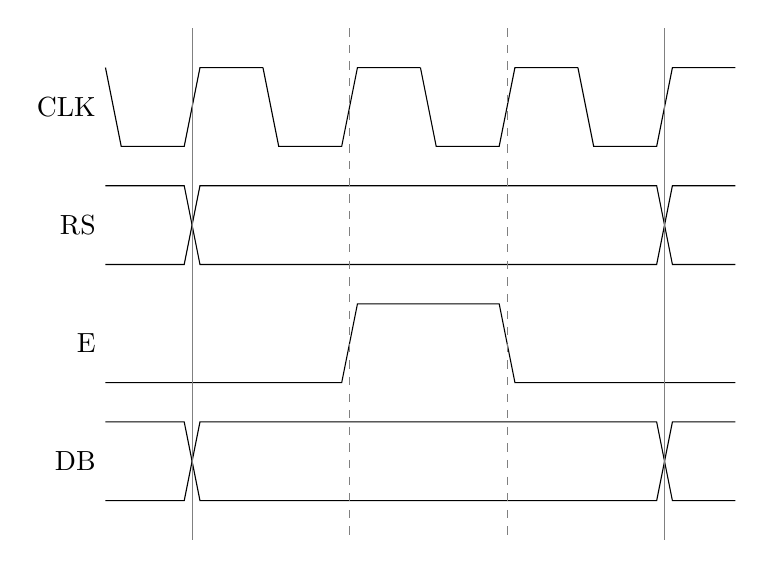
\begin{tikzpicture}
		\foreach \x in {0,2,4,6} \draw (\x-0.1,1) -- (\x+0.1,0) -- (\x+0.9,0) -- (\x+1.1,1) -- (\x+1.9,1);
		\draw (-0.1,-1.5) -- (0.9,-1.5) -- (1.1,-0.5) -- (6.9,-0.5) -- (7.1,-1.5) -- (7.9,-1.5);
		\draw (-0.1,-0.5) -- (0.9,-0.5) -- (1.1,-1.5) -- (6.9,-1.5) -- (7.1,-0.5) -- (7.9,-0.5);

		\draw (-0.1,-3.0) -- (2.9,-3.0) -- (3.1,-2.0) -- (4.9,-2.0) -- (5.1,-3.0) -- (7.9,-3.0);

		\draw (-0.1,-4.5) -- (0.9,-4.5) -- (1.1,-3.5) -- (6.9,-3.5) -- (7.1,-4.5) -- (7.9,-4.5);
		\draw (-0.1,-3.5) -- (0.9,-3.5) -- (1.1,-4.5) -- (6.9,-4.5) -- (7.1,-3.5) -- (7.9,-3.5);

		\node[left] at (-.1, 0.5) {CLK};
		\node[left] at (-.1,-1.0) {RS};
		\node[left] at (-.1,-2.5) {E};
		\node[left] at (-.1,-4.0) {DB};

		\draw[gray] (1,1.5) -- (1,-5);
		\draw[gray,dashed] (3,1.5) -- (3,-5);
		\draw[gray,dashed] (5,1.5) -- (5,-5);
		\draw[gray] (7,1.5) -- (7,-5);
	\end{tikzpicture}
\end{frame}

\begin{frame}{Display Driver Overview}
	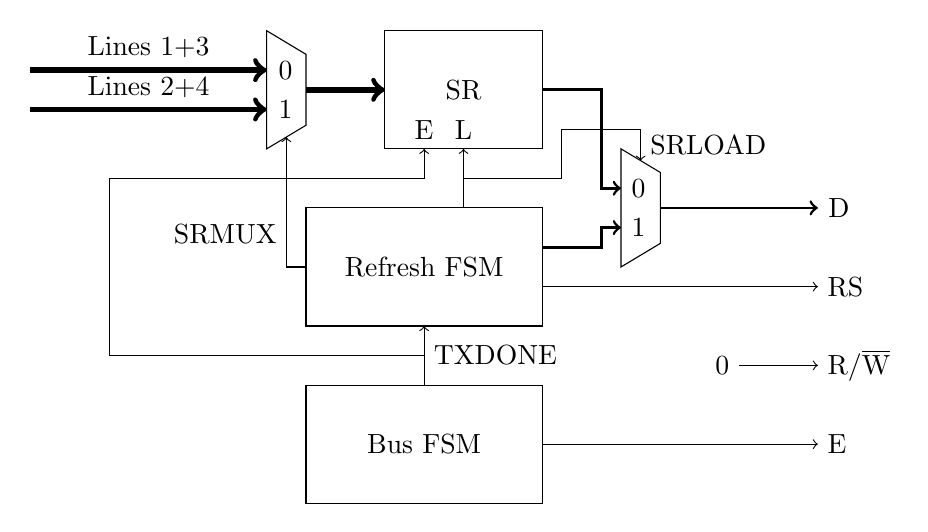
\begin{tikzpicture}
		\draw[line width=2pt,->] (0,0) -> (3, 0) node[midway,above] {Lines 1+3} node[right] {0};
		\draw[line width=2pt,->] (0,-.5) -> (3, -.5) node[midway,above] {Lines 2+4} node[right] {1};
		\draw[line width=2pt,->] (3.5,-.25) -> (4.5,-.25);
		\draw[line width=1pt,->] (6.5,-.25) -- (7.25,-.25) -- (7.25,-1.5) -> (7.5,-1.5) node[right] {0};
		\draw[line width=1pt,->] (6.5,-2.25) -- (7.25,-2.25) -- (7.25,-2) -> (7.5,-2) node[right] {1};
		\draw[line width=1pt,->] (8,-1.75) -> (10,-1.75) node[right] {D};

		\draw (3,.5) -- (3.5,.2) -- (3.5,-.7) -- (3,-1) -- cycle;

		\node at (5.5, -.25) {SR};
		\draw (4.5,.5) rectangle (6.5,-1);

		\node at(5,-2.5) {Refresh FSM};
		\draw (3.5,-1.75) rectangle (6.5,-3.25);

		\node at(5,-4.75) {Bus FSM};
		\draw (3.5,-4) rectangle (6.5,-5.5);

		\draw[->] (5,-4) -> (5,-3.25) node[right,midway] {TXDONE};
		\draw[->] (5,-3.625) -- (1,-3.625) -- (1,-1.375) -- (5, -1.375) -> (5, -1) node[above] { E };

		\draw[->] (3.5,-2.5) -- (3.25,-2.5) -> (3.25,-.85) node[left,near start] {SRMUX};

		\draw[->] (5.5,-1.75) -> (5.5,-1) node[above] {L};
		\draw[->] (5.5,-1.375) -- (6.75,-1.375) -- (6.75,-.75) -- (7.75,-.75) -> (7.75,-1.15) node[right,midway] {SRLOAD};

		\draw (7.5,-1.0) -- (8,-1.3) -- (8,-2.2) -- (7.5,-2.5) -- cycle;

		\draw[->] (6.5,-2.75) -> (10,-2.75) node[right] {RS};
		\draw[->] (6.5,-4.75) -> (10,-4.75) node[right] {E};
		\draw[->] (9,-3.75) node[left] {0} -> (10,-3.75) node[right] {R/$\overline{\text{W}}$};
	\end{tikzpicture}
\end{frame}

\begin{frame}{Display Driver Bus FSM}
	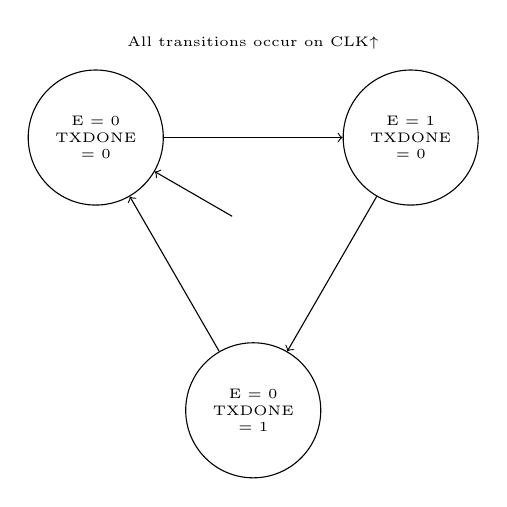
\begin{tikzpicture}[text width=1.3cm,align=center,font=\tiny,auto]
		\node[text width=4cm] at (2,1.2) {All transitions occur on CLK$\uparrow$};
		\node[state] (S0) at (0, 0) { E = 0 \\ TXDONE = 0 };
		\node[state] (S1) at (4, 0) { E = 1 \\ TXDONE = 0 };
		\node[state] (S2) at (2,-3.464102) { E = 0 \\ TXDONE = 1 };

		\path[->] (S0) edge (S1)
		          (S1) edge (S2)
		          (S2) edge (S0)
		          (S0) ++ (-30:2) edge (S0);
	\end{tikzpicture}
\end{frame}

\begin{frame}{Display Driver Refresh FSM}
	\begin{tikzpicture}[text width=1.3cm,align=center,font=\tiny,node distance=.5cm,auto]
		\node[right,text width=100cm,align=left] at (2,1.2) {All transitions occur on CLK$\uparrow$ if TXDONE = 1};
		\node[state]                       (FunctionSet)  { RS = 0 \\ D = 0x38 \\ SRMUX = X \\ SRLOAD = X };
		\node[state,right=of FunctionSet]  (DisplayOnOff) { RS = 0 \\ D = 0x0C \\ SRMUX = X \\ SRLOAD = X };
		\node[state,right=of DisplayOnOff] (SetAddrUpper) { RS = 0 \\ D = 0x80 \\ SRMUX = 0 \\ SRLOAD = 1 };
		\node[state,right=of SetAddrUpper] (WriteUpper)   { RS = 1 \\ D = X    \\ SRMUX = X \\ SRLOAD = 0 };
		\node[state,below=of WriteUpper]   (SetAddrLower) { RS = 0 \\ D = 0xC0 \\ SRMUX = 0 \\ SRLOAD = 1 };
		\node[state,left =of SetAddrLower] (WriteLower)   { RS = 1 \\ D = X    \\ SRMUX = X \\ SRLOAD = 0 };

		\path[->] (FunctionSet) ++(0,-2) edge (FunctionSet)
		          (FunctionSet)  edge                                  (DisplayOnOff)
		          (DisplayOnOff) edge                                  (SetAddrUpper)
		          (SetAddrUpper) edge                                  (WriteUpper)
		          (WriteUpper)   edge             node {SRDONE = 1}    (SetAddrLower)
		                         edge[loop right] node {SRDONE \\ = 0} ()
		          (SetAddrLower) edge                                  (WriteLower)
		          (WriteLower)   edge             node {SRDONE = 1}    (SetAddrUpper)
		                         edge[loop left]  node {SRDONE = 0}    ();
		\path[->,dashed]
		          (WriteLower)   edge                                  (FunctionSet);
	\end{tikzpicture}
\end{frame}

\begin{frame}[fragile]{Clock Buffer VHDL component}
\begin{verbatim}
type time_signals is record
  dayofweek:  unsigned(2 downto 0);
  [...]
  minute:     unsigned(6 downto 0);
  valid:      std_logic;
end record;

component time_buffer is
  port(
    uni:      in  universal_signals;
    time_in:  in  time_signals;
    time_out: out time_signals
  );
end component;
\end{verbatim}
\end{frame}

\begin{frame}{Clock Buffer Design}
	\begin{itemize}
		\item identical input and output format
		\item update internal registers if input is valid
		\item after 600000 cycles of invalid input, increment internal registers
		\item increment logic is a simple ripple-carry adder
		\item some logic to properly handle the day of the month
		\item consider 00 to not be a leap year
	\end{itemize}
\end{frame}

\end{document}
